\section{Reconstruction}
\label{sec:reconstructionmath}
The objective of this project is to compute a three dimensional reconstruction of an object by use of a camera, a rotation stage as well as a structured light source. The main idea behind this is to be able to find the depth of the object by detecting with the camera how the structured light is deformed over the surface of the object as a result of the object depth. The object is then rotated a full 360 degrees in order to get a full three dimensional reconstruction.\\

In order to construct a three dimensional model of a rotating object illuminated by structured light, it is first necessary to establish a mathematical model describing the relation between the depth of the object and the distortion of the structured light occurring due to the shape of the object surface. In this chapter basic trigonometric relations and knowledge of camera models will be used to establish such a mathematical model. Later, the overall test setup including the position and orientation of the camera, the object, the light source and the rotation stage will be illustrated. From this setup, a mathematical model will be proposed which can describe the relation between the object depth and the observed change in pixel coordinates of the structured light source projected onto the object.\\

Finally, the performance benefits and trade-offs of different camera, object and light source configurations will be discussed.  

\subsection{Camera models} \label{reconstruction:cameramodels}

In this report, a digital single-lens reflex (DSLR) camera is used to record footage of the rotating object. The lens on the front of the camera focuses light from the scene onto a light sensitive chip consisting of a number of pixels, yielding an image with a certain resolution. The lens, which is assumed thin, bends the oncoming light such that the two following properties are satisfied:

\begin{itemize}
    \item Light rays passing through the optical center of the lens are not affected by the lens.
    \item The light rays passing through parallel with the optical axis of the lens are bent such that they pass through the focal point.
\end{itemize}

These conditions form the thin lens model which is illustrated in figure \ref{fig:thinlensmodel}, where $f$ is the focal length of the lens.
\begin{figure}[h]
    \centering
    \includegraphics[width=0.7\textwidth]{figures/reconstruction/thinlensmodel2.pdf}
    \caption{Thin lens model}
    \label{fig:thinlensmodel}
\end{figure}

From figure \ref{fig:thinlensmodel} it can be seen that the light ray traced from the point $P$ through the optical center of the lens form the hypotenuses of two similar right-angled triangles with heights $A$ and $B$ as well as side lengths $a_{1}$ and $a_{2}$, respectively. These triangles are highlighted blue in figure \ref{fig:thinlensmodel}. Since these triangles are similar, it must hold that:

\begin{equation}
\label{eq:thinlens1}
    \frac{B}{A} = \frac{a_{1}}{a_{2}}
\end{equation}

Furthermore, we see from figure \ref{fig:thinlensmodel} that the light ray traced from the point $P$ parallel with the optical axis of the lens is directed through the focal point, forming the hypotenuses of another pair of similar right-angled triangles with the same heights $A$ and $B$ but with side lengths $f$ and $a_{2}-f$, respectively. These triangles are highlighted red in figure \ref{fig:thinlensmodel}. Given that this pair of right-angled triangles are also similar yields:

\begin{equation}
\label{eq:thinlens2}
    \frac{B}{A} = \frac{a_{2}-f}{f} = \frac{a_{2}}{f}-1
\end{equation}

Now, equating the right hand side of equations \ref{eq:thinlens1} and \ref{eq:thinlens2} yields the familiar thin lens equation \cite{imageformationDTU}:

\begin{equation}
\label{eq:thinlensequation}
    \frac{a_{1}}{a_{2}} = \frac{a_{2}}{f}-1 \Rightarrow \frac{1}{f} = \frac{1}{a_{1}} + \frac{1}{a_{2}}
\end{equation}

Which can be used to measure distances given the focal length and the distance $a_{2}$ is known. Further approximations, however, can still be made to the thin lens model given certain circumstances. Suppose that the object is very far away from the lens, this scenario is illustrated in figure \ref{fig:thinlensmodel_far}. 

\begin{figure}[h]
    \centering
    \includegraphics[width=0.8\textwidth]{figures/reconstruction/thinlensmodel3.pdf}
    \caption{Thin lens model far away}
    \label{fig:thinlensmodel_far}
\end{figure}

From figure \ref{fig:thinlensmodel_far} it can be seen that the further away the point $P$ is, the smaller the term $\frac{1}{a_{1}}$ in equation \ref{eq:thinlensequation} becomes and the closer the distance $a_{2}$ is to the actual focal length $f$. When $a_{1} >> f$ the thin lens equation is well approximated by:

\begin{equation}
    \frac{1}{f} = \frac{1}{a_{1}} + \frac{1}{a_{2}} \approx \frac{1}{a_{2}}
\end{equation}

Which is known as the pinhole approximation \cite{imageformationDTU}, an illustration of which can be seen in figure \ref{fig:pinhole_model}. In an ideal pinhole camera, the aperture size is assumed sufficiently small such that only a single light ray per world point is let through to hit the image plane. For this to be the case, however, all light rays must pass through the point $C$ which is called the optical center or center of projection. The resulting image appears sharp without the need of a lens. 

\begin{figure}[h]
    \centering
    \includegraphics[width=0.7\textwidth]{figures/reconstruction/pinhole_approx.pdf}
    \caption{pinhole camera approximation}
    \label{fig:pinhole_model}
\end{figure}

Looking at figure \ref{fig:pinhole_model} we can yet again utilize similar triangles to obtain a relation between the camera frame coordinates of the point $P=[X_{c}, 0, Z_{c}]$, the picture coordinate $x$ and the focal length $f$ \cite{imageformationDTU}:

\begin{equation}
\label{eq:Xc}
    -\frac{x}{X_{c}} = \frac{f}{Z_{c}} \Rightarrow x = -f  \frac{X_{c}}{Z_{c}}
\end{equation}

For the point with camera frame coordinates $P = [Y_{c}, 0, Z_{c}]$ we get similarly:

\begin{equation}
\label{eq:Yc}
    -\frac{y}{Y_{c}} = \frac{f}{Z_{c}} \Rightarrow y = -f  \frac{Y_{c}}{Z_{c}}
\end{equation}

Therefore, if the image plane coordinates $(x,y)$ of object are known as well as the camera frame coordinates of the object $(X_{c}, Y_{c})$, it is possible to estimate the distance $Z_{c}$ at which the object is located given that the focal length $f$ can also be found. The minus sign in equations \ref{eq:Xc} and \ref{eq:Yc} can be omitted for convenience since placing the image plane in front of the optical center yields the same result but a positive sign instead.\\  

The image plane coordinates $(x,y)$ are not directly readable from an image taken by a modern camera, since modern cameras digitize images into pixels yielding a set of pixel coordinates $(u,v)$. In figure \ref{fig:uvframe} an illustration is shown of how the pixel coordinates $(u,v)$ can be found when light from a point $P$ is projected onto the image plane of the camera. The blue dot in figure \ref{fig:uvframe} has pixel coordinates $(u_{0},v_{0})$ and marks the so-called principal point which lies in the center of the image plane.

\begin{figure}[h]
    \centering
    \includegraphics[width=0.7\textwidth]{figures/reconstruction/uvframe.pdf}
    \caption{pinhole camera approximation}
    \label{fig:uvframe}
\end{figure}

In order for equations \ref{eq:Yc} and \ref{eq:Xc} to become applicable, the image plane coordinates must be converted into pixel coordinates. The image plane coordinates $(x,y)$ and the pixel coordinates are related by a scaling factor $k_{u}$ and $k_{v}$ for $x$ and $y$, respectively. The scaling converts pixel distances into meters based on the inverse of the actual pixel size in meters along $x$ and $y$, which will of course vary from camera to camera based on the sensor resolution and the dimensions of the sensor inside the camera. The relation can be seen in equation \ref{eq:kukv}.
\begin{equation}
\label{eq:kukv}
    \begin{split}
        x & = u_{0} + k_{u} u\\
        y & = v_{0} + k_{v} v
    \end{split}
\end{equation}

Where $(u_{0},v_{0})$ is the principal point.\\ 

Combining the equations \ref{eq:kukv}, \ref{eq:Xc} and \ref{eq:Yc} and omitting the minus sign for convenience yields:

\begin{equation}
\label{eq:uv}
    \begin{split}
        u & = u_{0}+\frac{k_{u} f X_{c}}{Z_{c}} \\
        v & = v_{0}+\frac{k_{v} f Y_{c}}{Z_{c}}
    \end{split}
\end{equation}

Commonly, these equations are simplified to include the focal lengths in $x$ and $y$ expressed in pixels $f_{x}$ and $f_{y}$ which are simply found by multiplying the focal length with the scaling factors $k_{u}$ and $k_{v}$:
\begin{equation}
\label{eq:fxfy}
    \begin{split}
        f_{x} = k_{u} f\\
        f_{y} = k_{v} f
    \end{split}
\end{equation}

As will be explained later, the parameters $f_{x}$ and $f_{y}$ can be found directly from the camera calibration matrix $\boldsymbol{K}$. Thus, assuming the parameters $f_{x}$ and $f_{y}$ can be found as well as the inverse of the pixel size of the camera, the focal length may be computed.\\

In equations \ref{eq:Xc} and \ref{eq:Yc} it is assumed that either $X_{c}$ or $Y_{c}$ is known in order to find the depth $Z_{c}$. As these variables would in reality be unknown and given that only a single camera is used, meaning one cannot make use of stereo vision to find the distance, another mathematical model must be established to find the depth $Z_{c}$, which exploits knowledge about the general setup E.G the position and orientation of the camera, the laser and the rotation stage used in this report. In the following, a proposal for such a mathematical model will be presented.\\   

The experimental setup consists of an object, a structured light source, a rotation stage and a DSLR camera. The consisting parts of the setup are configured as seen in figure \ref{fig:setup1}.

\begin{figure}[h]
    \centering
    \includegraphics[width=0.9\textwidth]{figures/reconstruction/setup_2.pdf}
    \caption{Illustration of the experimental setup. The camera, object and structured light source are placed to form a right-angled triangle with side lengths $z$, $h$ and $b$. The camera forms the angle $\phi$ with the horizontal baseline $b$.}
    \label{fig:setup1}
\end{figure}

An object of interest is placed on a cylindrical rotation stage a distance $z$ from a structures light source. The object is placed as close to the center of the stage as possible.\\

Next, a camera is placed in a suitable distance $h$ from the object and oriented such that the principal point of the camera frame as close as possible aligns with the geometric center of the rotation stage. Furthermore, the height and pitch angle of the camera is adjusted such that the principal point of the camera frame closely matches the middle point of the object along the axis of rotation.\\

The structured light source is selected as a laser projecting a single narrow beam of light, which is then passed through a refractive element, creating a fan of light beams of lesser intensity. This fan of light beams is then pointed towards the object to be examined and adjusted such that the beams form a vertical dotted line perpendicular to the ground. Additionally, the fan of light beams is oriented such that the dotted line coincides with the geometric center of the rotation stage. More details about the setup can be found in section \ref{sec:experimental setup}.\\

With the rotation stage in the position of $0^{o}$, the yaw angle of the camera (the rotation about the axis pointing out of the paper) forms the nominal angle $\phi$ with the horizontal baseline $b$. Assuming the distances $z$, $b$ and $h$ are known, the angle $\phi$ is simply found by:
\begin{equation}
\label{eq:phi}
    \phi = \arctan{\left(\frac{z}{b}\right)}
\end{equation}

Assume next, however, that an object of varying depth is placed on the rotation stage and the stage is turned from $0^{o}$ to $90^{o}$. This scenario is illustrated in figure \ref{fig:depth_1}.  

\begin{figure}[h]
    \centering
    \includegraphics[width=0.8\textwidth]{figures/reconstruction/depthchange_v2.pdf}
    \caption{Illustration of how the depth $z'$ changes as the rotation stage moves from $0^{o}$ to $90^{o}$. The red diamond represents the object of interest seen from above}
    \label{fig:depth_1}
\end{figure}

When the object is rotated as seen in figure \ref{fig:depth_1}, because of the depth change of the object in the direction of the structured light, the light beams from the laser will strike the object at a distance $z'$ instead of the nominal distance $z$. This distance $z'$ forms a new triangle with the same baseline $b$, however, with a different angle denoted $\phi'$. The difference in angle is denoted $\theta$ such that:
\begin{equation}
\label{eq:phi'}
    \phi' = \phi - \theta
\end{equation}
Assuming therefore that this difference in angle $\theta$ can be found it will be possible through simple trigonometry to compute the unknown distance $z'$ needed to find the depth $d$ of the object.
\begin{equation}
\label{eq:z'}
    z' = b \tan(\phi') = b \tan(\phi - \theta)
\end{equation}
\begin{equation}
\label{eq:d}
    d = z - z'
\end{equation}
Looking from the camera's point of view, the rotation will appear to have shifted some or all of the vertical laser dots to the left in the image plane (or visa versa to the right if the depth of the object has gotten "thinner" at the point where the structured light hit the object). This shift occurs because of the perspective or angle at which the camera is looking at the object. In fact, the movement of the laser points will follow a set of epipolar lines originating from the structured light source. Because the fan of laser beams originate from a single point, as can be seen in the left illustration in figure \ref{fig:setup1}, these lines will be close to but not be exactly parallel with the ground. Therefore, when the object as a result of it's own depth moves closer to the light source, the laser points will appear to move slightly down in the image plane looking from the camera's perspective. An illustration showing this phenomenon can be seen in figure \ref{fig:ly} where the epipolar lines in the image plane have been exaggerated for clarification. These epipolar lines can then be used to track the laser points from frame to frame assuming that the epipolar line slope can found.\\   

\begin{figure}[h]
    \centering
    \includegraphics[width=0.8\textwidth]{figures/reconstruction/ly.pdf}
    \caption{Illustration showing the dots moving along their each respective epipolar line.}
    \label{fig:ly}
\end{figure}

In conclusion, there will be both a measurable change in pixel coordinates in $u$ and $v$ when the object is rotated. In this report, however, it is assumed that the change in pixel coordinates along $v$ has negligible impact on the estimation of the depth. This approximation is fair assuming the maximum depth change of the object is much smaller than the distance $z$ or in other words; the structured light source is located very far away and the size of the object is a small fraction of this distance.\\

The measurable horizontal distance $l_{x}$ in pixel coordinates in the image plane is illustrated in figure \ref{fig:2frames}. The left frame illustrates the nominal case when the shift in pixel coordinates of the laser points in the horizontal direction is zero, which would correspond to a depth change of zero I.E $z' = z$. Keep in mind the nominal case only occurs when an object of zero depth is placed on the rotation stage, for example a piece of paper.  

\begin{figure}[h]
    \centering
    \includegraphics[width=0.8\textwidth]{figures/reconstruction/2frames.pdf}
    \caption{Illustration of the change in pixel coordinates as seen from the camera's point of view. Some or all of the laser points' pixel coordinates along the $u$-axis will shift when the object rotates while being illuminated by the structured light source.}
    \label{fig:2frames}
\end{figure}

In order to find a relation between the distance $l_{x}$ and the angle $\theta$, the pinhole camera approximation model seen in figure \ref{fig:pinhole_model} can now be used. An illustration showing the point $P$ being projected onto the image plane of a pinhole camera can be seen in figure \ref{fig:lxfig} along with the distance $l_{x}$ as well as the angle $\theta$.\\  

\begin{figure}[h]
    \centering
    \includegraphics[width=0.8\textwidth]{figures/reconstruction/lxfig.pdf}
    \caption{Illustration of how the light from a laser point $P$ projects onto the image plane of a pinhole camera, resulting in two similar right-angled triangles with the same angle $\theta$. The distance $l_{x}$ can be directly measured as the distance from the principal point to pixel coordinates of the laser point in the image frame.}
    \label{fig:lxfig}
\end{figure}

Looking at figure \ref{fig:lxfig} it can be seen that the projection of the light from the point $P$ onto the image plane forms two similar right-angled triangles in the plane defined by the camera frame basis vectors $(X_{c}, Z_{c})$. The angle between the $Z_{c}$-axis of the camera frame and the projection line of $P$ is exactly the angle $\theta$ also depicted in figure \ref{fig:depth_1}. Now, since the two right-angled triangles seen in figure \ref{fig:lxfig} are similar, the angle $\theta$ may be found by equation \ref{eq:theta}:

\begin{equation}
\label{eq:theta}
    \theta = \arctan\left(\frac{l_{x} }{k_{u} f}\right)
\end{equation}

Where the factor $k_{u}$ is added to convert the distance $l_{x}$ from pixels to meters.\\

The next step is to find the height of the object according to the height of the laser point in the image plane. Recall first the fact that the depth $Z_{c}$ in the camera frame is in fact equal to the hypothenuse of the right-angled triangle seen in figure \ref{fig:depth_1} whose angle is equal to $\phi'$. Therefore, the distance $Z_{c}$ can simply be found using Pythagoras theorem as:
\begin{equation}
\label{eq:pythagoran_zc}
    z_{c} = \sqrt{b^{2} + z'^{\;2}}
\end{equation}
Next, the height $Y_{c}$ can be found by inserting the appropriate values inside equation \ref{eq:uv}.\\

In general, the height in the camera coordinate frame may not be same as in the world coordinate frame. Thus in order to find a corresponding height for the found depth $d$, a conversion is needed which relates the camera and world frame. The exact relation between the camera frame coordinates and the world coordinate frame can found as result of both a translation $\boldsymbol{T}$ and rotation $\boldsymbol{R}$ of the world frame coordinates $(X_{w}, Y_{w}, Z_{w})$:
\begin{equation}
    \boldsymbol{P_{c}} = \boldsymbol{R} \boldsymbol{P_{w}} + \boldsymbol{T}
\end{equation}
Similarly from the world to camera frame we have:
\begin{equation}
    \boldsymbol{P_{w}} = (\boldsymbol{P_{c}} - \boldsymbol{T})\boldsymbol{R}^{-1}
\end{equation}

In the specific case of the setup illustrated in figure \ref{fig:setup1}, it will however be assumed that $y$-axis the camera frame perfectly coincides with the $y$-axis of the world frame and therefore, no conversion is needed.\\  

In order to reconstruct the object as a point cloud in 3D space, the depth values found using equations \ref{eq:theta}, \ref{eq:z'}, \ref{eq:d} as well as the height points are stores as vectors. These vectors are then rotated by the same angle as the rotation stage position for each frame. An illustration showing the rotation of the point vectors in 3D space can be seen in figure \ref{fig:pointcloud}. Assuming the object is rotating with angular velocity $\omega$ and a recording is taken with a frame rate of $F$ frames per second, the necessary rotation angle $\psi(i)$ for frame $i$ is:

\begin{equation}
    \psi(i) = i\frac{\omega}{F} \hspace{1cm} i = 0..N=\frac{2\pi F}{\omega}
\end{equation}
Where it is further assumed that the rotation begins on frame 0 of the recording.

\begin{figure}[h]
    \centering
    \includegraphics[width=0.8\textwidth]{figures/reconstruction/pointcloud.pdf}
    \caption{Illustration of the point vectors observed in frame $i$ being rotated around the $y$-axis to create the 3D reconstruction of the object. The red points form the point cloud of the object.}
    \label{fig:pointcloud}
\end{figure}

The world coordinates of point $P_{i}$ observed in frame $i$ can thus be reconstructed as

\begin{equation}
    P_{i} =  \begin{bmatrix}
    d \sin(\psi(i)) \\
    Y_{c} \\
    d \cos(\psi(i))  \\
    \end{bmatrix}
\end{equation}
where $d$ is the depth of the point found using equation \ref{eq:d}.\\

Now that a mathematical model of estimating the depth of the rotating object has been established, it is of interest to investigate how precise the depth can actually be determined. In this regard, there are many sources of error which will be investigated later in report. For instance, accurate estimation of the centroid of the laser points on the object has a large impact, since the lower the variance of centroid algorithm, the less noisy the depth estimate will be. From a theoretical stand point however, the major factor constraining the precision is the location of the camera, object and light source, or in other words, how the setup seen in figure \ref{fig:setup1} is configured. A motivating example of this could be that for instance having the object closer to the camera will increase the size of the image plane which the object covers and therefore, changes in the position of laser points on the object will be easier to detect. Of course, having the object closer may have other trade offs; For example there may be more radial distortion of the object in the far corners of the image plane or the camera may need to have a larger field of view in order to have all of the object inside the frame.\\

The precision factor which will be investigated is the camera angle $\phi$ and how altering this angle may affect depth estimation. Suppose that the camera is placed in two different configurations with angles $\phi_{1}$ and $\phi_{2}$ such that: 
\begin{equation}
\begin{split}
    \phi'_{1} = \phi_{1} - \theta_{1} \hspace{1cm}
    \phi'_{2} = \phi_{2} - \theta_{2} \hspace{1cm}
    \phi_{1} > \phi_{2}
\end{split}
\end{equation}
An illustration showing these two configurations of the test setup using different camera angles can be seen in figure \ref{fig:variationangle}, note that the length $h$ is the same in both cases.\\

\begin{figure}[h]
    \centering
    \includegraphics[width=0.9\textwidth]{figures/reconstruction/variationangle.pdf}
    \caption{Illustration of two different camera configurations. In the left subplot, the camera forms the angle $\phi_{1}$ from the lines sections $h$ to $b_{1}$. In the right subplot the camera forms the angle $\phi_{2}$. The distance $h$ from the object to the camera is the same for both configurations}
    \label{fig:variationangle}
\end{figure}

Looking at figure \ref{fig:variationangle} it can be seen that decreasing the angle $\phi$ results in the same depth change yielding different angles $\theta_{1}$ and $\theta_{2}$ where $\theta_{1} < \theta_{2}$ from the camera's point of view. Therefore, assuming the pinhole camera model illustrated in figure \ref{fig:lxfig} is good approximation of the real camera system, the larger value $\theta_{2}$ will also result in a larger value for the distance $l_{x}$. Since the same depth change can be explained by a larger value for $l_{x}$ it must also hold that the depth resolution I.E the minimum depth change which can be explained by a single pixel, is increased. To illustrate this point using a quantitative measure, a three dimensional plot showing how the depth varies as a function of the pixel distance $u$ and the camera angle $\phi$ in degrees can be seen in figure \ref{fig:maplefig1}.\\   

\begin{figure}[H]
    \centering
    \includegraphics[width=0.6\textwidth]{figures/reconstruction/maplefig1_crop.pdf}
    \caption{Plot of the depth $d$ of the object as a function of both the camera angle $\phi$ and the distance from the principal point in pixels $u$. The distance from the object to the camera is found using Pythagoras theorem with $z = 1.136$m and $b=0.649$m.}
    \label{fig:maplefig1}
\end{figure}

Looking at the surface seen in figure \ref{fig:maplefig1}, it can be seen that the angle $\phi$ has a huge impact on the perceived depth. As $\phi$ grows larger, the facing of the camera becomes more parallel to the light source, which results in lower depth resolution. In other word, each pixel corresponds to a larger variation in the depth. When the angle $\phi$ approaches 90 degrees, the relation between $d$ and $u$ becomes highly non-linear. Furthermore, $d \rightarrow \infty$ when $\phi \rightarrow \pi/2$ and the depth reconstruction becomes impossible.\\ 

Conversely, when the angle $\phi$ is small, the depth resolution becomes larger and larger. Additionally, as the angle $\phi$ gets smaller, the relation between $d$ and $u$ becomes approximately proportional. This is not surprising, as when the camera looks at the object from a completely perpendicular point of view, the depth change becomes completely proportional to the distance $l_{x}$. The depth is then explained completely by $l_{x}$, the factor $k_{u}$ and the focal length $f$.\\

In figure \ref{fig:maplefig2} the depth $d$ is plotted as a function of the pixel distance $u$ for four different angles of $\phi$.

\begin{figure}[H]
    \centering
    \includegraphics[width=0.6\textwidth]{figures/reconstruction/maplefig2_crop.pdf}
    \caption{Plot of $d$ of the object as a function of the distance from the principal point in pixels $u$. The distance from the object to the camera is same as in figure \ref{fig:maplefig1}. Each line in the plot corresponds to a different $\phi$.}
    \label{fig:maplefig2}
\end{figure}

It can be again seen from figure \ref{fig:maplefig2} that a smaller angle results in a more proportional relationship between $d$ and $u$ as well as better depth resolution.\\

To quantify the depth resolution achievable at different camera angles, figure \ref{fig:maplefig3} shows a plot of the depth $d$ change corresponding to a single pixel as a function of $\phi$. 

\begin{figure}[H]
    \centering
    \includegraphics[width=0.6\textwidth]{figures/reconstruction/maplefig_res_crop.pdf}
    \caption{Plot of depth change in millimeters corresponding to a single pixel as a function of the camera angle $\phi$. The distance from the object to the camera is same as in figure \ref{fig:maplefig1}}
    \label{fig:maplefig3}
\end{figure}

Looking at figure \ref{fig:maplefig3} it can be seen that the depth resolution, as expected, increases when the angle $\phi$ decreases. The relation, as can be seen, is highly non-linear with the depth $d$ approaching infinity when the camera angle approaches 90 degrees.\\

One may be tempted to think from the plots seen in figures \ref{fig:maplefig1}, \ref{fig:maplefig2} and \ref{fig:maplefig3} that choosing the angle $\phi$ as small as possible is the most optimal solution. There is, however, one major problem with this: occlusions.\\

In order for the depth of the object to be measured when rotated, the laser dots projected onto the object must be visible from the camera's point of view. For objects with little depth variation like for example a cylinder, this is not a problem since no matter the angle $\phi$ the camera will be able to see the laser dots regardless of the rotation angle of the stage. For objects with large depth variation, however, this becomes a problem since the object itself has a risk of occluding the laser dots from the camera. A situation like this is illustrated in figure \ref{fig:occlusion} where two different setup configurations are shown along with the camera field of view cones from two different angles. Looking at figure \ref{fig:occlusion} it can be seen that the depth of the object shadows the part of the object where the laser light is supposed to hit when the camera is placed with the angle $\phi_{2}$. Therefore, the depth cannot be determined and part of the reconstruction will be missing.\\

Now, the camera is instead placed with the angle $\phi_{1}$ as also seen in figure \ref{fig:occlusion}. In this situation since the camera is significantly more parallel with the facing of the light source, the object will not shadow the laser dots and the depth can be successfully determined. As such, when the camera is moved such that the angle $\phi$ becomes larger, the maximum allowed depth variation increases. 
\begin{figure}[h]
    \centering
    \includegraphics[width=0.6\textwidth]{figures/reconstruction/occlusion.pdf}
    \caption{Illustration of two different camera configuration shown overlapping each other. The distance from the object to the camera is held constant while the angle of the camera facing is changed from $\phi_{1}$ to $\phi_{2}$.}
    \label{fig:occlusion}
\end{figure}
 
In conclusion, when configuring the test setup there is a performance trade-off between maximum allowed object depth and depth resolution. From figure \ref{fig:occlusion} it can be seen that objects with very large depth variations require a larger camera angle which in turn means the reconstruction will have lower resolution. On the other hand, if the object is close to cylindrical, the camera angle can be selected smaller such that very small variations in depth can be successfully detected.\\

So far it has been established that the object can in fact be reconstructed in 3D implying the laser points being projected onto the object can actually be detected. Furthermore, if the dots can be detected, the desired depth resolution can be achieved as a trade-off of lowering the maximum allowed depth variation of the object. There is problem with this method, however, in that every single laser only gives information about the depth at the points where the light hits the object. This means that for every dot it is only possible to reconstruct the object depth in a horizontal plane as a result of the object completing a full rotation. The object depth is essentially discretized along the vertical axis yielding a series of horizontal planes giving the rough outline of the object when factoring in all the laser dots. An illustration of this can be seen in figure \ref{fig:scanlines}. As a result of this discretization, any depth variation in between the planes cannot be reconstructed.\\

\begin{figure}[h]
    \centering
    \includegraphics[width=0.8\textwidth]{figures/reconstruction/scanlines.pdf}
    \caption{Illustration of how the depth reconstruction along the vertical axis becomes discretized into horizontal planes, giving a rough outline of the object shape.}
    \label{fig:scanlines}
\end{figure}

In order to achieve a better resolution along the vertical axis of the object, ones first suggestion would be to reduce the distance between each laser dot being projected onto the object such that the distance between each horizontal plane of depth can be lowered, yielding a higher fidelity reconstruction. This can be done by using another refractive filter in front of the laser with a higher line density. The main problem with this approach of adding more laser dots is that detection of each individual laser point becomes more and more difficult.\\

When light from the laser hits the object, due to both imperfections in the refractive filter in front of the laser and the reflective properties of the surface of the object, the light will not be perfectly structured into equally sized dots. Instead, the light from each dot will in fact bleed out a bit. As a result, if the density of laser dots is sufficiently high, the light from the laser dots will bleed into one another and can cause confusion for the algorithm that tries to estimate the centroid of each individual dot. An illustration of this can be seen in figure \ref{fig:dotdensity}.     

\begin{figure}[h]
    \centering
    \includegraphics[width=0.8\textwidth]{figures/reconstruction/dotdensity.pdf}
    \caption{Illustration of two different configurations of the structured light source. Using different refractive elements in front of the laser yields more or less laser points which can cause confusion between the dots themselves.}
    \label{fig:dotdensity}
\end{figure}

In conclusion, a refractive element should be used with yields the highest possible density of the laser dots without causing confusion for the algorithm used to find the centroid for each dot. 

\newpage 
 
 
\iffalse
\begin{itemize}
    \item Pinhole model
    \item Setup (camera, laser, rotating platform, environment (good and bad video, background)) (outside picture frame), also difference between 1st and 2nd data collection
    \item Scene analysis (center of rotation, signal2noise ratio, laser dot shape, how to handle occlusion, how big angle of light source vs camera position to get greater angle vs occlusion, resolution of scan, precision, how much does centroiding invariance correspond to changes in depth)
    (inside picture frame)


    \item Depth and other derivations from setup
    \item Sensor, specs, deriving focal length
    \item Point cloud
    \item code for point cloud stuff, flowcharts
    \item Polygon mesh
\end{itemize}
\fi

\subsection{Experimental setup}
\label{sec:experimental setup}
The experimental setup for gathering data are set up as described in figure \ref{fig:setup1}. The camera and the laser are approximately lined up, forming a right-angled triangle with the rotating stage.\\

The laser is a HLM1230 5mW red laser module from Batchen \cite{laserDatasheet}. It uses less than 5mW of power and has a wavelength of 650 nm. In the test setup, it was powered by a regular lab power supply, adjusted to meet the specifications of the data sheet. A refracting element was mounted in front with some tape, converting the single laser beam, into a line consistinc of many smaller ones. This was the source of the structured light. \\

To capture the images, a Canon 2000D EOS DSLR with a EFS 18-55 mm lens was used. This camera has a sensor size of approx. 22.3 mm x 14.9 mm (type CMOS), 3:2 aspect ratio \cite{canonCamera}. The camera was controlled through DigiCam Control using a Windows computer. \\

To rotate the object of choice, the M-062 rotating stage \cite{rotationStage} using a C-863 controller\cite{rotationStageController} by Physik Instrumente (P.I.) was used. It was controlled using proprietary software developed by P.I. \\

The complete setup can be seen in figure \ref{fig:testsetup_world}. 
\begin{figure}[h]
    \centering
    \includegraphics[width=0.9\textwidth]{figures/reconstruction/IMG_0001.JPG}
    \caption{Experimental setup. Stand rotates with object upon, while the camera records. The camera was moved slightly before the data was collected.}
    \label{fig:testsetup_world}
\end{figure}

This is actually version 2 of the setup, as the first data collection had some issues with glare from the laser that created a bleeding effect around each dot. This is described more in depth in section \ref{imageanalysis:problemoutline}. Also, to try and increase the signal to noise ratio, a black background was added. All the lights in the room were turned off for both data collections, but for the second one it was also dark outside. 
The camera was placed at an appropriate angle. \\

The method for collecting data is: 1) zoom camera so object fills as much as possible in the frame, and adjust values such that object is in focus and clearly visible, 2) start recording video, 3) let the stand rotate slowly until one full rotation has been completed. This was done exactly as described for both data collections. 


A few different iterations of data collection were done, but only the two best were kept. They are referred to as data collection 1 and 2. \\

The main object to be scanned is a cross, and not the multimeter seen in figure \ref{fig:testsetup_world} sitting on the rotating stage. 

\subsection{Scene analysis}
In order to make sure that the collected data is "good enough" to analyse and do further work on, a scene analysis must be done first. The primary goal of this analysis will be to ensure that the signal to noise ratio is high. The analysis will mainly be done for the second data collection, as this one improved upon a few of the mistakes that were made. \\

The second data collection uses a black background with all the lights in room turned off, while it's dark outside. Given that the dots are red, there should be a nice contrast. A typical frame from the video can be seen in figure \ref{fig:cross2basic}.
\FloatBarrier
\begin{figure}[h]
        \centering
        \includegraphics[width=0.9\textwidth]{figures/ImageAnalysis/cross2_base.png}
        \caption{2nd data collection. Typical frame.}
        \label{fig:cross2basic}
        % frame number 5
\end{figure}

As can be seen from figure \ref{fig:cross2basic}, the dot are clearly visible with high contrast and good amount of color variation. There occurs glare and therefore bleeding, but it is mostly in a part of the image which wont be used for analysis (the stage the object is sitting on). The histogram for this cropped frame (with no glare) is plotted in figure \ref{fig:cross2basehistcropped}.
\FloatBarrier
\begin{figure}[h]
        \centering
        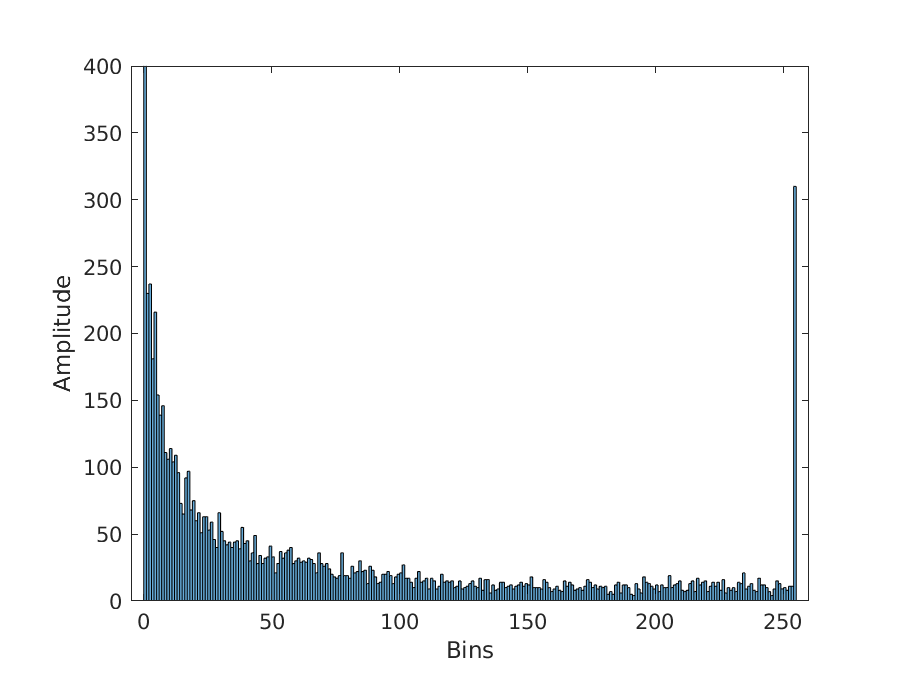
\includegraphics[width=0.7\textwidth]{figures/reconstruction/base2_cropped_histogram.eps}
        \caption{2nd data collection. Histogram of red component of typical frame, but cropped to not include the glare and bleeding happening at the bottom of the image. Y-axis has been scaled down to $400$. Peak value of bin [0,1] is $4.885050 \cdot 10^6$.}
        \label{fig:cross2basehistcropped}
        % frame number 5
\end{figure}
\FloatBarrier
Looking at the histogram, one might expect a bump around a certain bin value, but as it turns out, about everything above a value of 10 is actually color and light coming from the dots, see figure \ref{fig:base2_thresholded}. This means that there is good seperation between bagground and foreground. 
\begin{figure}[h]
    \centering
    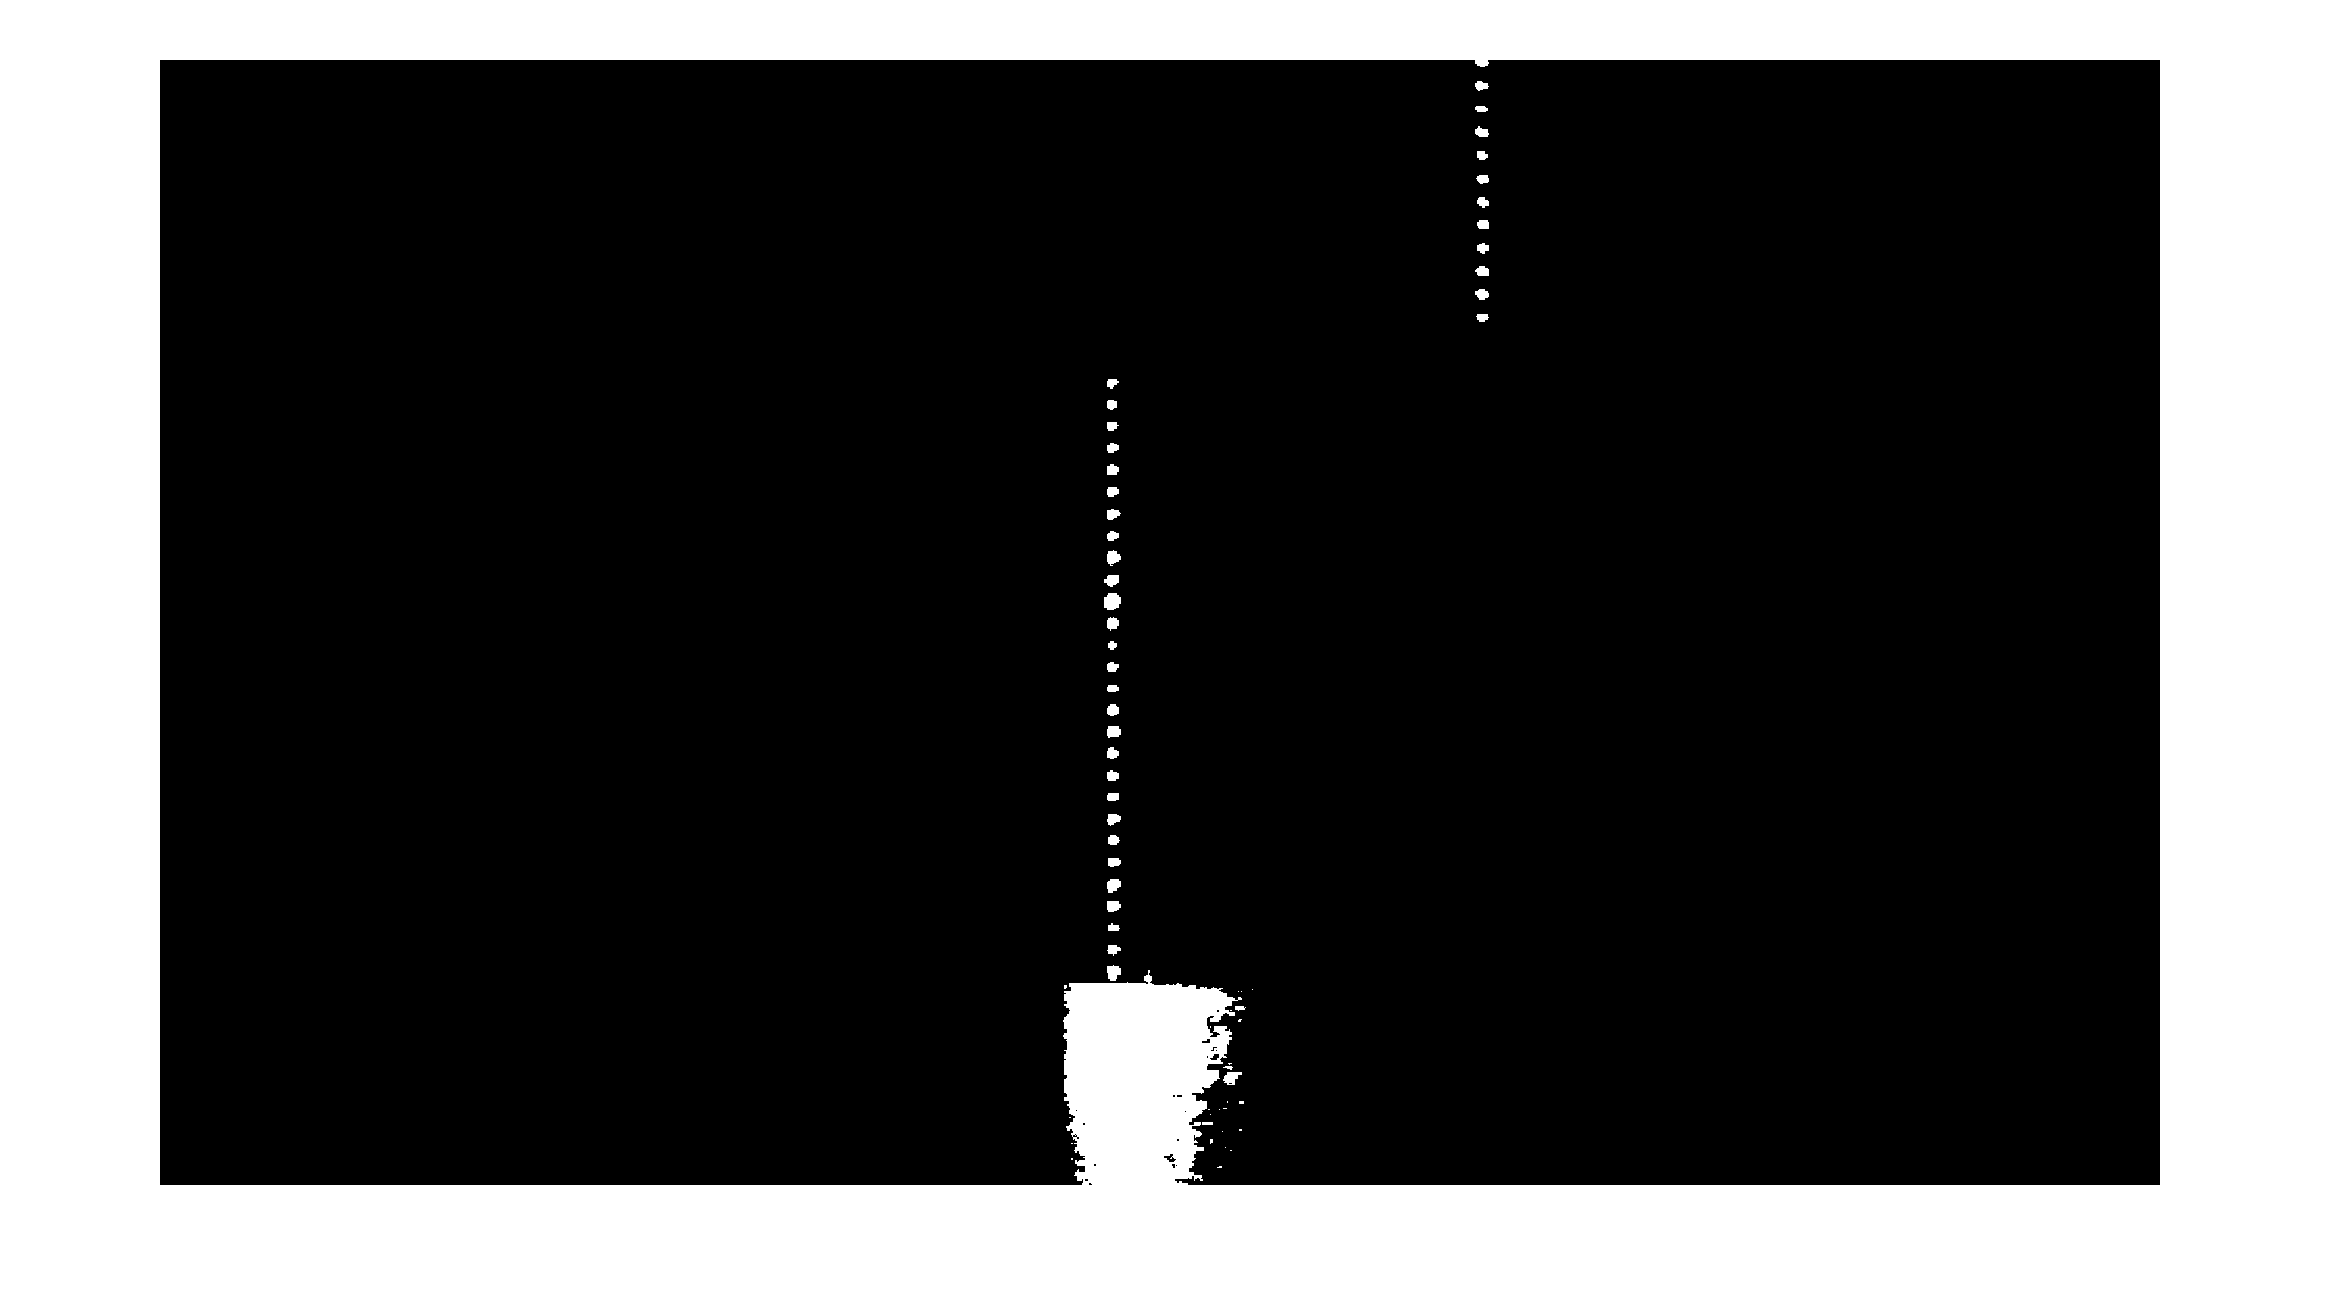
\includegraphics[width=0.5\textwidth]{figures/reconstruction/base2_thresholded.eps}
    \caption{Same frame as figure \ref{fig:cross2basic}, but was a grayscale image thresholded at a value of 10. }
    \label{fig:base2_thresholded}
\end{figure}
When glare occurs, and red color from the dot centers starts bleeding out, the histogram looks very similar, except there is a higher amount of white light in the image. The signal to noise ratio is still good, and the dots can be extracted with the right choice of method. Though, there are certain cases where the saturation level of the dots is very low, but the dots can still be extracted even though the ratio is slightly worse. This is also discussed in section \ref{imageanalysis:problemoutline}. \\


The epipolar lines are found by mapping lines that connect dots between two frames. Because the laser is so far away, the lines can be approximated with parallel horizontal lines. This is also useful when extracting dots and detecting outliers. 

